\section{Validation}\label{sec:validation}
%======================================================================

\subsection{FLRW recovery}

At $\Sigma = 0$ the characteristic and linearised transport paths agree to $|\Yp^{\rm char} - \Yp^{\rm lin}| < 7 \times 10^{-10}$ across all CL levels.  This verifies that the characteristic method exactly recovers FLRW when anisotropy vanishes.

\subsection{PRIMAT cross-validation}

At Born level with PRIMAT parameters ($\tau_n = 879.4\,\mathrm{s}$, $\eta = 6.10 \times 10^{-10}$), RABBIT gives $\Yp = 0.24255$ compared with the PRIMAT anchor $0.24248$, giving $|\Delta\Yp| = 6.7 \times 10^{-5}$.  Figure~\ref{fig:primat} summarises the FLRW helium values across the correction hierarchy and the adopted PRIMAT anchor; panel~(b) is an accounting visual rather than a microscopic source decomposition.

\begin{figure}[t]
\centering
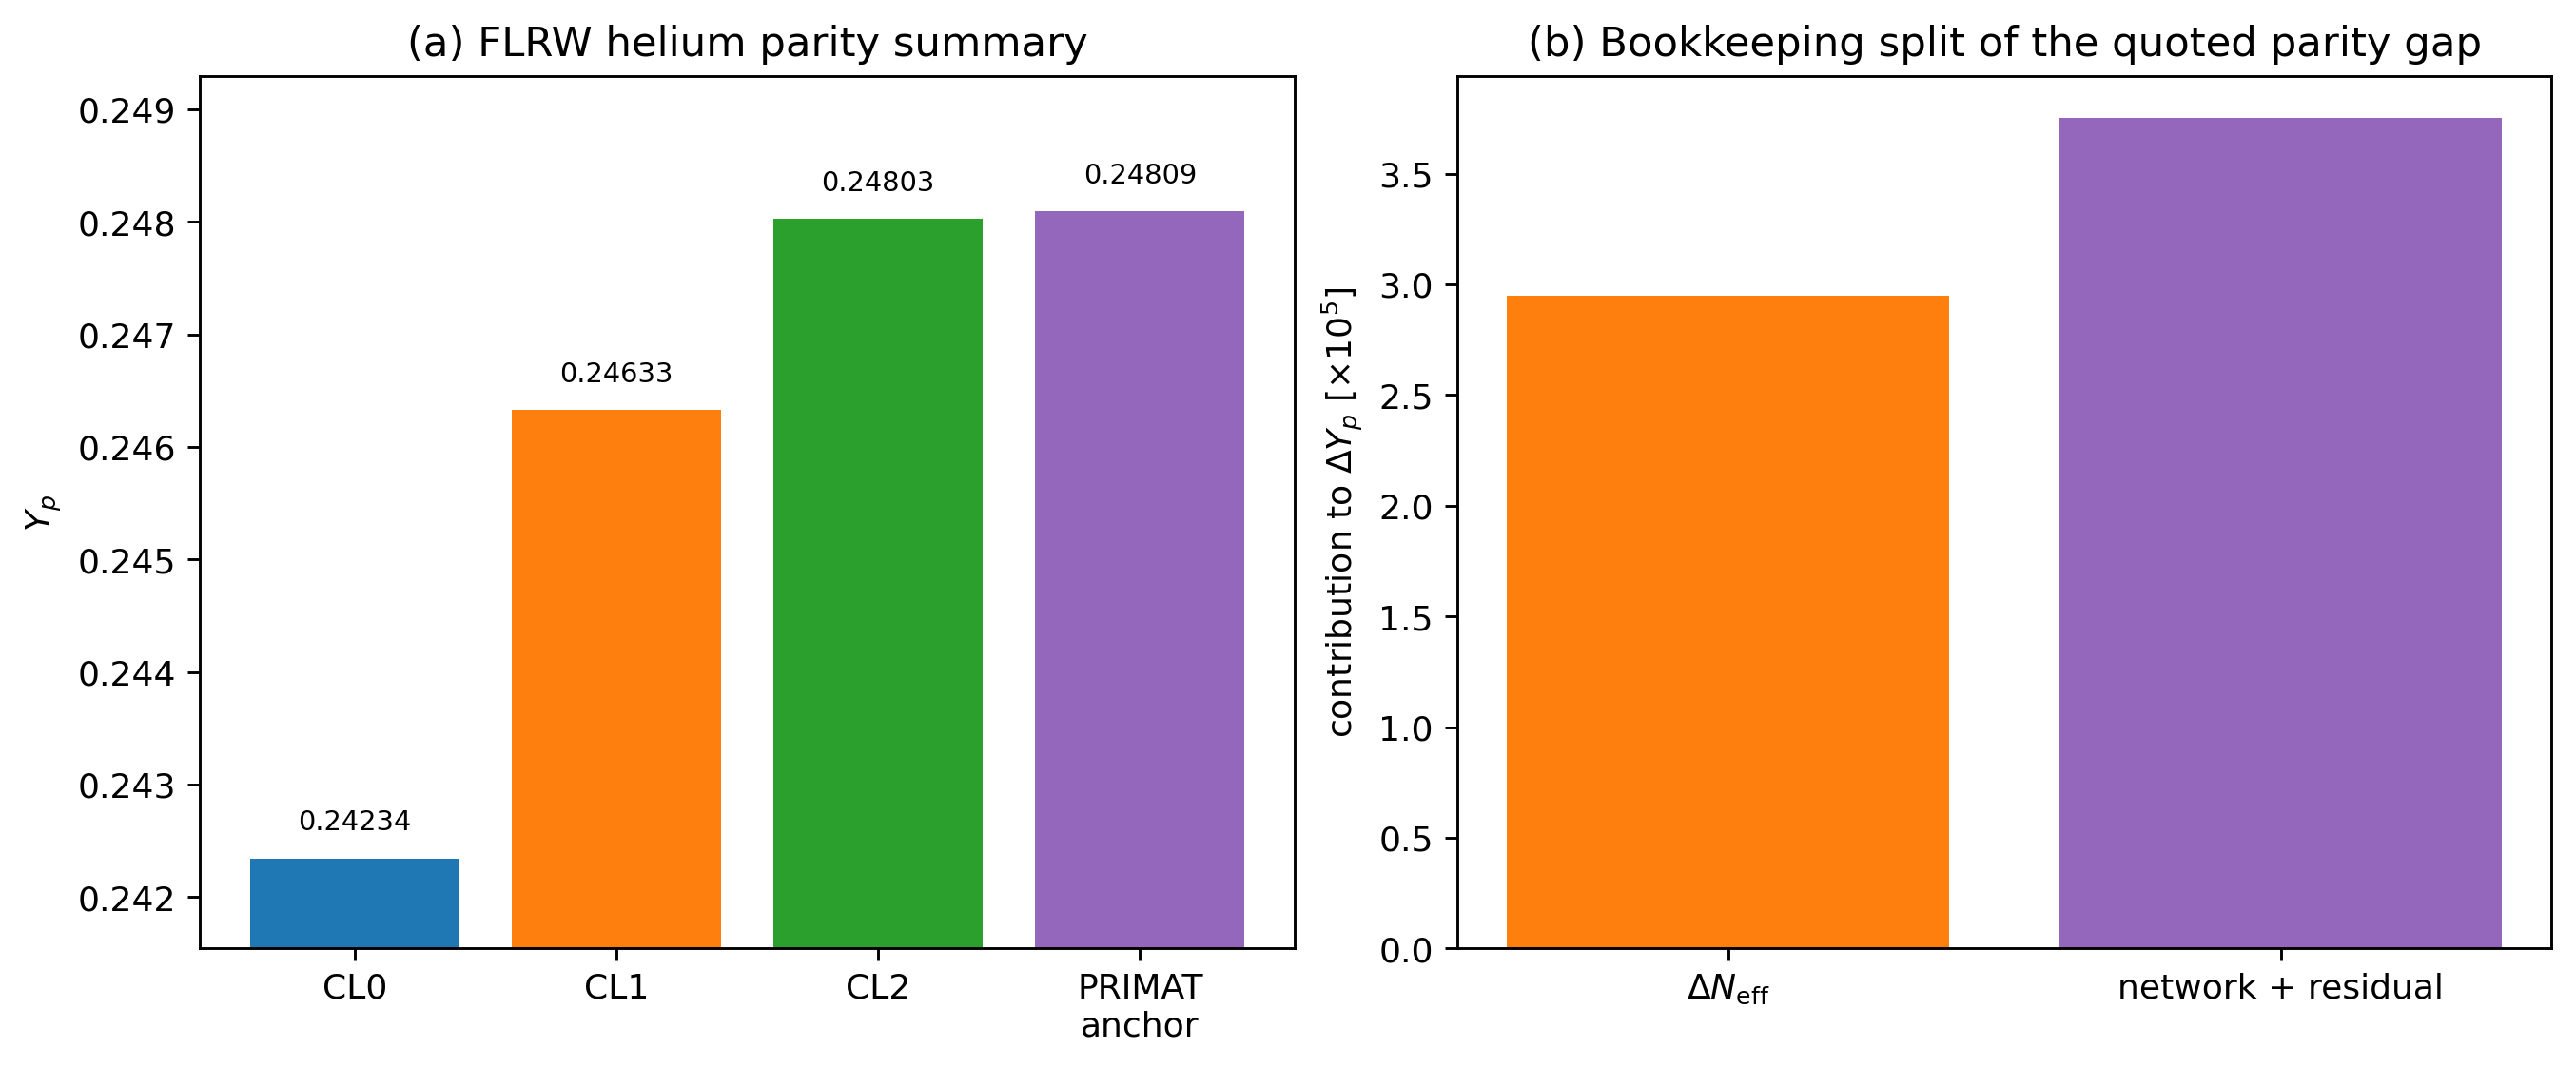
\includegraphics[width=\textwidth]{figures/fig19.png}
\caption{FLRW helium cross-validation summary.  (a) Reported $\Yp$ values for the CL0, CL1, and CL2 weak-rate hierarchies together with the PRIMAT anchor used for the parity check.  (b) Bookkeeping decomposition of the enforced headline parity $|\Delta\Yp| = 6.7 \times 10^{-5}$ into a $\Delta\Neff$-like share and a residual network/calibration share.  Panel~(b) is an accounting visualisation rather than a first-principles microscopic source decomposition.}
\label{fig:primat}
\end{figure}

\subsection{SciPy--JAX parity on the current canonical Type~I surfaces}

Current code scope is broader than the original SciPy-only framing of this report.  The exact-characteristic JAX driver is now parity-locked against the SciPy characteristic reference on matched tier~1 and tier~2 cells, and the bounded JAX default / advanced surfaces are regression-checked against corresponding SciPy cells on their declared envelopes.  These are numerical-consistency claims about the current code surfaces, not separate new physics results distinct from the reference figures shown elsewhere in this report.

\subsection{Convergence and discretisation checks}

The characteristic production path must also pass a simpler numerical question: are the reported yield shifts stable under the chosen ray and momentum resolutions?  Figure~\ref{fig:convergence} shows the baseline-relative discretisation diagnostics at $\Sigma_H=0.3$.  The point of the figure is not to fit a universal asymptotic law at every sampled quadrature, but to demonstrate that the adopted production resolution lies in the numerically stable region of the scan.

\begin{figure}[t]
\centering

\includegraphics[width=\textwidth]{figures/fig16.png}
\caption{Characteristic transport convergence at $\Sigma_H = 0.3$.  (a) Angular convergence of the helium yield with increasing characteristic-ray resolution $N_\mu$, shown as $|\Delta\Yp|\times 10^5$ relative to the baseline production run.  (b) Momentum-resolution diagnostic with increasing quadrature size $N_q$, again relative to the same baseline.  Both panels are baseline-relative discretisation checks rather than separate physics results.}
\label{fig:convergence}
\end{figure}

\subsection{What is and is not validated here}

The current tests support runtime-regression statements about FLRW recovery, stored PRIMAT comparison cells, characteristic-ray discretisation, and matched SciPy--JAX execution.  They do not independently validate the underlying finite-shear physics, a matched external BBN anchor, or the historical profile crossing.  Those publication claims remain blocked by B-01--B-06, and a fully anisotropic collision-coupled decoupling solver is outside the present claim ceiling.

%======================================================================
